\documentclass{article}
\usepackage{amsmath}
\usepackage{amssymb}
\usepackage{tikz}
\usepackage[utf8]{inputenc}
\usepackage{float}

\usepackage[a4paper]{geometry}
\geometry{top=1.5cm, bottom=3.0cm, left=1.25cm, right=1.25cm}

\usetikzlibrary{shapes ,arrows}


\title{TP N$^\circ$2 \\ Sistemas controlados por computadora}
\author{Saez, Lautaro Andres}
\date{}

\newcommand{\laplaceTransform}[1]{\mathcal{L}\left\{ #1 \right\}}
\newcommand{\syseq}[1]{ \left\{  
                            \begin{array}{c}
                                #1
                            \end{array}
                        \right. }

\begin{document}
    \maketitle
  

    \tikzstyle{block} = [draw, fill=blue!20, rectangle, 
    minimum height=3em, minimum width=6em]
    \tikzstyle{sum} = [draw, fill=blue!20, circle, node distance=1cm]
    \tikzstyle{input} = [coordinate]
    \tikzstyle{output} = [coordinate]
    \tikzstyle{pinstyle} = [pin edge={to-,thin,black}]
    \tikzstyle{big-block} = [draw, rectangle, minimum height= 12em, minimum width= 24em]

    \section{Ejercicio 1}

    \subsection{a)}

    El sistema para discretizar en este caso es 

    \begin{equation}
        \left\{
            \begin{array}{c}
                \dot{x} = \underbrace{
                        \begin{pmatrix}
                            0 & 1 \\
                            -1 & 0 
                        \end{pmatrix}
                        }_{A} x +
                        \underbrace{
                            \begin{pmatrix}
                                0 \\ 1
                            \end{pmatrix}
                        }_{B} u \\ 
                y = \underbrace{
                    \begin{pmatrix}
                        0 & 1
                    \end{pmatrix}
                }_{C} x
            \end{array}
        \right.
    \end{equation}

    Para discretizar el sistema primero debemos calcular $e^{At}$, en general utilizaremos la transforma inversa de Laplace salvo que la matriz $A$ sea 
    diagonalizable, para ello calculo los autovalores de $A$

    \begin{equation}
        p(\lambda) = |A-\lambda I| = \lambda^2 + 1
    \end{equation}

    Cuyas raices son $\lambda \in \{ \pm j \}$. Luego calcularemos los espacios asociados a cada autovalor utilizando la siguiente relación 

    \begin{equation}
        (A-\lambda_i I) 
        \begin{pmatrix}
            x \\ y    
        \end{pmatrix}
        = 
        \begin{pmatrix}
            0 \\ 0
        \end{pmatrix}
    \end{equation}

    Remplazando 

    \begin{equation}
        x = \mp j y
    \end{equation}

    Para armar la matriz de transformación que diagonalice a $A$ elijo 1 autovector de cada espacio. Por lo tanto

    \begin{equation}
        T = \begin{bmatrix}
            1 & 1 \\
            j & -j
        \end{bmatrix}
    \end{equation}

    Ahora es posible calcular $e^{At}$ como 

    \begin{equation}
        e^{At} = T e^{\Lambda t} T^{-1}
    \end{equation}

    Donde $\Lambda$ es una matriz diagonal compuesta por lo autovalores de $A$. Realizando las cuentas se obtiene 

    \begin{equation}
        e^{At} = \frac{1}{2} 
        \begin{bmatrix}
            \cos{t} & \sin{t} \\ 
            -\sin{t} & \cos{t} 
        \end{bmatrix}
    \end{equation}

    Finalmente las matrices discretizadas son 

    \begin{equation}
        \begin{array}{c}
            \Phi = e^{Ah} \\ 
        \Gamma = \int_0^h e^{Al}dl B
        \end{array}
    \end{equation}

    Donde $\Phi$ es la versión discretizada de $A$, y $\Gamma$ la versión discretizada $B$, las matrices $C$ y $D$ no se ven modificadas.

    Por lo que el sistema discretizado es 

    \begin{equation}
        x[k+1] = 
        \underbrace{
            \frac{1}{2}
            \begin{bmatrix}
                \cos{h} & \sin{h} \\ 
                -\sin{h} & \cos{h}   
            \end{bmatrix}
        }_{\Phi} x[k] + 
        \underbrace{
            \frac{1}{2}
            \begin{bmatrix}
                1 - \cos{h} \\ 
                \sin{h}
            \end{bmatrix}
        }_{\Gamma} u[k]
    \end{equation}

    \subsection{b)}
        El sistema a tratar es 

        \begin{equation}
            \ddot{y} + 3 \dot{y} + 2 y = \dot{u} + 3u
        \end{equation}

        Aplicando la transformada de Laplace obtenemos 

        \begin{equation}
            (s^{2} + 3s + 2)Y(s) = (s + 3)U(s)
        \end{equation}

        Por lo tanto la transferencia $G(s)$ es 

        \begin{equation}
            G(s) = \frac{s+3}{s^2 + 3s + 2}
        \end{equation}

        Si descrizamos con un mantenedor de orden cero la transferencia discreta se puede escribir como 

        \begin{equation}
            H(z) = (1-z^{-1})\mathcal{Z}\left\{ \left. \laplaceTransform{ \frac{G(s)}{s} }\right|_{t=hk} \right\}
        \end{equation}

        Como primer paso calcularemos $G(s)/s$ por lo que tenemos 

        \begin{equation}
            \frac{G(s)}{s} = \frac{s+3}{( s+2 )(s+1)s} = \frac{A}{s} + \frac{B}{s+2} + \frac{C}{s+1}
        \end{equation}

        De la ecuación anterior surgue el siguiente sistemas de ecuaciones 

        \begin{equation}
            \left\{
                \begin{array}{c}
                    A+B+C = 0 \\
                    3A + B + 2C = 1 \\
                    2A = 3
                \end{array}    
            \right.
            \Leftrightarrow
            \syseq{
                A = \frac{3}{2} \\ 
                B = \frac{1}{2} \\
                C = -2
            }   
        \end{equation}

        Antitransformando la respuesta al escalon obtenemos 

        \begin{equation}
            q(t) = \frac{1}{2} \left( 3 + e^{-2t} - 4e^{-t} \right)\mu(t)
        \end{equation}

        La versión discretizada que se obtiene es 

        \begin{equation}
            q[k] = \frac{1}{2} \left( 3 + \alpha_0^k - 4 \alpha_1^k \right) \mu[k], \alpha_i = e^{-(2 - i)h}
        \end{equation}

        Finalmente si transformamos la expresión anterior 

        \begin{equation}
            G(z) = \frac{( 1 - z^{-1} )}{2} 
            \left( 
                \frac{3}{1 - z^{-1}} 
                + \frac{1}{1 - \alpha_0z^{-1}}
                - \frac{4}{1 - \alpha_1z^{-1}}
            \right)
        \end{equation}

        Al trabajar la expresión anterior obtenemos 

        \begin{equation}
            \syseq{
                G(z) = \frac{1}{2}\frac{az + b}{z^2 - ( \alpha_0 + \alpha_1 )z + \alpha_0\alpha_1}\\
                a=\alpha_0 -4\alpha_1+3\\
                b=3\alpha_{-1}-4\alpha_0+\alpha_1
            }
        \end{equation}

    \subsection{c)}
    
        En este inciso el sistema esta descripto por 

        \begin{equation}
            \dddot{ y } = u
        \end{equation}

        Realizando el mismo procedimiento que en el inciso anterior se obtiene 

        \begin{eqnarray}
            \left\{
                \begin{array}{c}
                    \dot{x} = 
                    \begin{bmatrix}
                        0 & 1 & 0 \\
                        0 & 0 & 1 \\
                        0 & 0 & 0 \\
                    \end{bmatrix} x +
                    \begin{bmatrix}
                        0 \\ 0 \\ 1
                    \end{bmatrix} u\\ 
                    y = 
                        \begin{bmatrix}
                            1 & 0 & 0
                        \end{bmatrix} x
                \end{array}
            \right.
        \end{eqnarray}

        Por simple inspección visual se puede determinar que $0$ es polo triple, al calcular el espacio asoaciado a dicho autovalor 
        se obtiene que es de dimensión 1, por lo tanto no es posible diagonalizar a $A$, por ello en este caso utilizaremos la transferencia de Laplace para calular
        $e^{At}$

        \begin{eqnarray}
            \mathcal{L} \{ e^{At} \} = (sI - A)^{-1}
        \end{eqnarray}

        Por lo tanto 

        \begin{eqnarray}
            \mathcal{L} \{ e^{At} \} = 
            \begin{bmatrix}
                s & -1 & 0 \\
                0 & s & -1 \\
                0 & 0 & s    
            \end{bmatrix}^{-1}
        \end{eqnarray}

        Una forma posible de calular la inversa es utilizando la adjunta, donde se obtiene 

        \begin{eqnarray}
            \mathcal{L} \{ e^{At} \} = 
            \begin{bmatrix}
                s^{-1} & s^{-2} & s^{-3} \\ 
                0   & s^{-1} & s^{-2} \\ 
                0 & 0 & s^{-1}
            \end{bmatrix}
        \end{eqnarray}

        Antitransofrando 

        \begin{eqnarray}
            e^{At} = \begin{bmatrix}
                1 & t & \frac{1}{2}t^2 \\ 
                0 & 1 & t \\
                0 & 0 & 1 
            \end{bmatrix}
        \end{eqnarray}


        Para la matriz $\Gamma$ realizaremos el mismo producto que en el inciso $b)$ con la finalidad de simplificar cuentas 

        \begin{eqnarray}
            e^{At}B = 
            \begin{bmatrix}
                h^2 \\ h \\ 1     
            \end{bmatrix}
        \end{eqnarray}


        Por lo tanto 

        \begin{eqnarray}
            \begin{array}{c}
                \Phi = 
                \begin{bmatrix}
                    1 & h & \frac{1}{2}h^2 \\ 
                    0 & 1 & h \\
                    0 & 0 & 1 
                \end{bmatrix} \\ 
                \Gamma = 
                \begin{bmatrix}
                    \frac{1}{6} t^{3} \\ \frac{1}{2} t^{2} \\ t
                \end{bmatrix}
            \end{array}
        \end{eqnarray}

    \section{Ejercicio 2}

        Un integrador doble puede ser escrito como 

        \begin{equation}
            \ddot{ y } = u
        \end{equation}

        Al pasarlo a variables de estado se obtiene 

        \begin{equation}
            \left\{
                \begin{array}{c}
                    \dot{x} = 
                        \begin{bmatrix}
                            0 & 1 \\ 
                            0 & 0
                        \end{bmatrix} x + 
                        \begin{bmatrix}
                            0 \\ 1
                        \end{bmatrix} u
                    \\ 
                    y = \begin{bmatrix}
                        1 & 0
                    \end{bmatrix} x
                \end{array}
            \right.
        \end{equation}

        Para expresar al sistema en su forma canonica controlable primero debemos discretizar el mismo. Pero
        al igual que el inciso 1-c, el cual es un integrador triple, no es posible diagonalizar la matriz $A$, por lo tanto recuriremos al calculo mediante la transfromada de Laplace 

        \begin{equation}
            \laplaceTransform{e^{At}} = 
                \begin{bmatrix}
                    s & -1 \\ 
                    0 & s 
                \end{bmatrix}^{-1}=
                \begin{bmatrix}
                    s^{-1} & s^{-2} \\ 
                    0 & s^{-1}
                \end{bmatrix}
        \end{equation} 

        Por lo tanto 

        \begin{equation}
            e^{At} = 
                \begin{bmatrix}
                    1 & t \\
                    0 & 1
                \end{bmatrix}
        \end{equation}

        Finalmente se tiene que 

        \begin{equation}
            \begin{array}{c}
                \Phi = 
                    \begin{bmatrix}
                        1 & h \\
                        0 & 1
                    \end{bmatrix} \\ 
                \Gamma = 
                    \begin{bmatrix}
                        \frac{1}{2} h^2 \\ h
                    \end{bmatrix}
            \end{array}
        \end{equation}

        Por lo tnto 

        \begin{equation}
            W_c = \frac{1}{2} 
            \begin{bmatrix}
                h^2 & 3h^2 \\ 
                2h & 2h
            \end{bmatrix}
        \end{equation}

        El determinante de la matriz $W_c$ que se obtiene es 

        \begin{equation}
            |W_c| = -h^3
        \end{equation}

        El cual es simpre distinto de $0$ salvo que $h=0$, pero si intrepretamos $h$ como el periodo de muestro del sistema este siempre debe ser mayor a $0$. Por lo tanto 
        siempre es posible escribir al sistema en su forma canonica controlable.

        Ahora sabemos que las matrices $\Gamma$ y $\Phi$ en forma canocia deberían ser de la forma 

        \begin{equation}
            \begin{array}{c}
                \Phi^\prime = 
                    \begin{bmatrix}
                        2 & -1 \\ 
                        1 & 0
                    \end{bmatrix}\\
                \Gamma^\prime = 
                    \begin{bmatrix}
                        1 \\ 0
                    \end{bmatrix}
            \end{array}
        \end{equation}

        Si planteamos la transformacion $z[k] = Tx[k]$, es posible encontrar las siguientes relaciones 

        \begin{equation}
            \syseq{
                z[k+1] = T^{-1}\Phi T z[k] + T^{-1}\Gamma u[k] \\ 
                y[k] = C T z[k]    
            }
        \end{equation}

        Luego 

        \begin{equation}
            \syseq{
                T^{-1}\Phi T = \Phi^\prime \\ 
                T^{-1}\Gamma = \Gamma^\prime
            }
        \end{equation}

        Con la finalidad de no expresar la matriz $T^{-1}$ ya que puede ser un poco engorroso y sabiendo que existe $T$, es decir, 
        la inversa de $T^{-1}$, podemos expresar el sistema anterios como 

        \begin{equation}
            \syseq{ 
                \Phi T = T \Phi^\prime \\
                \Gamma = T \Gamma^\prime
            }
        \end{equation}

        Luego proponemos 

        \begin{equation}
            T = 
                \begin{bmatrix}
                    a & b \\ 
                    c & d
                \end{bmatrix}
        \end{equation}

        Y realizando los productos matriciales obtenemos 

        \begin{equation}
            \syseq{
                \begin{bmatrix}
                    a + hc & b + hd \\
                    c & d
                \end{bmatrix} = 
                \begin{bmatrix}
                    2a+b & -a \\ 
                    2c+d & -c
                \end{bmatrix} \\
                \begin{bmatrix}
                    h^2/2 \\ 
                    h
                \end{bmatrix} = 
                \begin{bmatrix}
                    a \\
                    c
                \end{bmatrix}
            }
        \end{equation}

        Por lo que se tienen las siguientes ecuaciones 

        \begin{equation}
            \syseq{
                a = h^2/2 \\ 
                b = h \\
                a + hc = 2a + b \\
                b+hd = -a \\
                c=2c+d \\
                d = -c
            }
        \end{equation}

        Al resolver el sistema de ecuacionesanterior se obtiene 

        \begin{equation}
            a = \frac{h^2}{2}, b = \frac{h^2}{2}, c=h, d=-h
        \end{equation}

        Por lo tanto 

        \begin{equation}
            T = \frac{h}{2}
                \begin{bmatrix}
                    h & h \\
                    2 & -2 
                \end{bmatrix}
        \end{equation}

    \section{Ejercicio 3}

    El sistema esta descripto por 

    \begin{equation}
        \left\{
            \begin{array}{c}
                \dot{x} = -ax + bu \\
                y = cx
            \end{array}    
        \right.
    \end{equation}

    El polo del sistema es claramente $-a$, si calculamos la transferencia del sistema obtenemos 

    \begin{equation}
        G(s) = \frac{cb}{s + a}
    \end{equation}

    \subsection{a)}

    En este caso el calculo de $\Phi$ y $\Gamma$ no tiene mayor complejidad debido a que son escalares, por lo tanto 

    \begin{equation}
        \left\{
            \begin{array}{c}
                \Phi = e^{-ah} \\ 
                \Gamma = -\frac{b}{a} ( e^{-ah} - 1 )
            \end{array}
        \right.
    \end{equation}

    Por lo tanto la transferencia del sistema discretizada es 

    \begin{equation}
        H(z) = \frac{c\Gamma}{z-\Phi} = -\frac{cb}{a} \frac{e^{-ah}-1}{z - e^{-ah}}
    \end{equation}

    Donde el polo del sistema discretizado queda ubicado en $e^{-ah}$. 

    \subsection{b)}

    Como se observo en el inciso anterior la ubicación del polo en función de $h$ queda definido como $e^{-ah}$, por lo tanto 
    si el sistema continuo es estable podemos observar que el sistema discreto es inestable y viceversa.
    
    \subsection{c)}

    De la función $G(s)$ podemos calcular la respuesta al escalon 

    \begin{equation}
        Y(s) = \frac{G(s)}{s} = \frac{cb}{(s+a)s} 
    \end{equation}

    Planteando fracciones simples 

    \begin{equation}
        \frac{cb}{(s+a)s} = \frac{A}{s} + \frac{B}{s+a}
    \end{equation}

    Por lo que podemos plantear 

    \begin{equation}
        \left\{
            \begin{array}{c}
                A + B = 0 \\
                Ba = cb
            \end{array}
        \right.
        \Leftrightarrow
        \left\{
            \begin{array}{c}
                A = - \frac{cb}{a} \\ 
                B = \frac{cb}{a}
            \end{array}
        \right.
    \end{equation}

    Por lo tanto la respuesta es 

    \begin{equation}
        y(t) = -\frac{cb}{a} ( e^{-at} - 1 ) \mu(t)
    \end{equation}

    Por otro lado la respuesta en tiempo discreto es 

    \begin{equation}
        Y(z) = -\frac{cb}{a} \frac{(e^{-ah}-1)z}{(z - e^{-ah})(z-1) } 
    \end{equation}

    Al plantear fracciones simples

    \begin{equation}
        \frac{(e^{-ah}-1)z}{(z - e^{-ah})(z-1) } = \frac{A}{z - e^{-ah}} + \frac{B}{z - 1}
    \end{equation}

    \begin{equation}
        \left\{
            \begin{array}{c}
                A + B = e^{-ah} - 1 \\ 
                -A - Be^{-ah} = 0
            \end{array}
        \right.
        \Leftrightarrow
        \left\{
            \begin{array}{c}
                A = e^{-ah} \\ 
                B = -1
            \end{array}
        \right.
    \end{equation}

    Por lo tanto 

    \begin{equation}
        y[k] = -\frac{cb}{a} ( e^{-ahk} - 1 ) \mu[k-1]
    \end{equation}

     \begin{figure}[!htb]
         \centering
         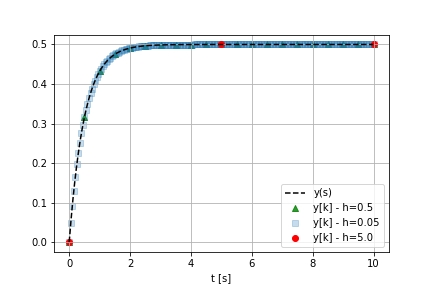
\includegraphics[width=\textwidth]{Img/3-c.png}
         \caption{Grafico de la respuesta al escalon del sistema discretizado para diferentes valores de $h$ junto con la respuesta del sistema continuo.}
         \label{}
     \end{figure}

    \section{Ejercicio 4}

        Para un filtro FIR de la siguiente forma 

        \begin{equation}
            \label{eq:ej4}
            H(z) = \sum_i^n b_{n-i}z^{-i}
        \end{equation}

        \subsection{a)}

            El orden del sistema es $n$.

        \subsection{b)}

            La forma observable esta definida como 

            \begin{equation}
                \syseq{
                    x[k+1] = 
                        \begin{bmatrix}
                            -a_1 & 1 & 0 & \cdots & 0 \\
                            -a_2 & 0 & \ddots & 0 & \cdots \\
                            \vdots & 0 & \cdots & \ddots & 0\\
                            -a_n & 0 & \cdots & 0 & 1\\
                        \end{bmatrix} x[k] + 
                        \begin{bmatrix}
                            b_1 \\
                            b_2 \\ 
                            \vdots \\ 
                            b_n
                        \end{bmatrix}u[k] \\
                    y[k] = 
                        \begin{bmatrix}
                            1 & 0 & \cdots & 0\\
                        \end{bmatrix}
                }
            \end{equation}

            En este caso como no tenemos polos no nulos o no infinitos los coefientes $a_i$ son nulos mientras que los $b_i$ estan dados por la ecuacion \ref{eq:ej4}.

            \begin{equation}
                \syseq{
                    x[k+1] = 
                        \begin{bmatrix}
                            0 & 1 & 0 & \cdots & 0 \\
                            0 & 0 & \ddots & 0 & \cdots \\
                            \vdots & 0 & \cdots & \ddots & 0\\
                            0 & 0 & \cdots & 0 & 1\\
                        \end{bmatrix} x[k] + 
                        \begin{bmatrix}
                            b_1 \\
                            b_2 \\ 
                            \vdots \\ 
                            b_n
                        \end{bmatrix}u[k] \\
                    y[k] = 
                        \begin{bmatrix}
                            1 & 0 & \cdots & 0\\
                        \end{bmatrix}
                }
            \end{equation}

    \section{Ejercicio 5}

        En este ejercicio se trabajara con la transferencia 

        \begin{equation}
            H(z) = \frac{K}{z(z-0.2)(z-0.4)}
        \end{equation}

        Si retroalimentamos negativamente el sistema se obtiene la siguiente transferencia 

        \begin{equation}
            G(z) = \frac{K}{z(z-0.2)(z-0.4) + K}
        \end{equation}

        Por lo tanto el polinomio caracteristo es 

        \begin{equation}
            z^3 - \frac{3}{5} z^2 + \frac{2}{25} z + K
        \end{equation}

        Aplicando el criterio de Jury 

        \subsection{Calculo de $a^2_i$}

            \begin{equation}
                a^3 = a^3_3 / a^3_0 = K
            \end{equation}

            Luego obtenemos que 

            \begin{equation}
                a^2_0 = a^3_0 - a^3a^3_3 = 1 - K^2
            \end{equation}

            \begin{equation}
                a^2_1 = a^3_1 - a^3a^3_2 = -\frac{3}{5} - \frac{2}{25} K 
            \end{equation}

           

        \subsection{Calculo de $a^1_i$}

            \begin{equation}
                a^2 = \frac{a^2_2}{a^2_0} = 
            \end{equation}

        \begin{table}
            \centering
            \begin{tabular}{|c|c|c|c|} 
                $1$ & $-3/5$ & $2/25$ & K \\
                $1-K^2$ & $-\frac{15+2K}{25}$ & $\frac{2+15K}{25}$ \\
                
            \end{tabular}
        \end{table}

    \section{Ejercicio 6}

            Para este problema se tiene el siguiente sistema 

            \begin{figure}[H]
                \centering
                \begin{tikzpicture}[node distance=2.5cm,auto,>=latex']
                    \node [input, name=input] {};
                    \node [sum, right of=input] (sum) {$+$};
                    \node [block, right of=sum] (controller) {$Kz^{-n_0}$};
                    \node [block, right of=controller, node distance=3.5cm] (DAC) {DAC};
                    \node [block, right of =DAC, node distance=3.5cm] (system) { $\frac{1}{S}$ };
    
                    \draw [->] (controller) -- node[name=u] { $U(z)$ } (DAC);
                    \draw [->] (DAC) -- node[name=u] { $U(s)$ } (system);
                    \node [output, right of=system] (output) {};
                    \node [block, below of=DAC] (H) {ADC};
                    
                    \draw [draw, ->] (input) -- node {$R(z)$} (sum); 
                    \draw [->] (sum) -- node {$E(z)$} (controller);
                    \draw [->] (system) -- node[name=y] {$Y(s)$} (output);
                    \draw [-] (y)  |- (H);    
                    \draw [->] (H) -| node[pos=0.99] {$-$} (sum);
                \end{tikzpicture}
                \caption{Diagrama del proceso.}
                \label{}
            \end{figure}

            Donde $n_0$ es $\tau=n_0h$.

            Es posible pensar al proceso muestreado por un mantenedor de orden cero, dando como resultado
            
            \begin{figure}[H]
                \centering
                \begin{tikzpicture}[node distance=2.5cm,auto,>=latex']
                    \node [input, name=input] {};
                    \node [sum, right of=input] (sum) {$+$};
                    \node [block, right of=sum] (controller) {$Kz^{-n_0}$};
                    \node [block, right of =controller, node distance=3.5cm] (system) { $\frac{1}{z-1}$ };
    
                    \draw [->] (controller) -- node[name=u] { $U(z)$ } (system);
                    \node [output, right of=system] (output) {};
                    \node [output, below of=system] (H) {};
                    
                    \draw [draw, ->] (input) -- node {$R(z)$} (sum); 
                    \draw [->] (sum) -- node {$E(z)$} (controller);
                    \draw [->] (system) -- node[name=y] {$Y(z)$} (output);
                    \draw [-] (y)  |- (H);    
                    \draw [->] (H) -| node[pos=0.99] {$-$} (sum);
                \end{tikzpicture}
                \caption{Diagrama del proceso.}
                \label{}
            \end{figure}

            Por lo tanto la tranferencia total del sistema retroalimentamo es 

            \begin{equation}
                H(z) = \frac{K}{z^{n_0+1} - z^{n_0} + K }
            \end{equation}

            \subsection{a)}

                Para este ejercicio tomaremos $n_0 \in \{0,1\}$.

                \subsubsection{$n_0=0$}

                    En este caso el ecuacion caracterisca del sistema esta dada por 

                    \begin{equation}
                        P(\lambda) = \lambda + ( K -1 )
                    \end{equation}

                    Donde el polo esta dado por la ecuacion 

                    \begin{equation}
                        p = 1 - K
                    \end{equation}

                    Para un sistema discreto la estabilidad esta dada cuando $|p|<1$, por lo tanto 

                    \begin{equation}
                        |1 - K| < 1
                    \end{equation}

                    Por lo cual obtenemos que $K \in ( 0 ; 2 )$

                \subsubsection{$n_0=1$}

                    En este caso el retardo es unitario por lo tanto el polinomio caracteristo esta dado por 

                    \begin{equation}
                        P(\lambda) = \lambda^2 - \lambda + K
                    \end{equation}

                    En este caso para calcular cuando el sistema es estable aplicaremos el criterio de Jury

                    \begin{table}[H]
                        \centering
                        \begin{tabular}{|c|c|c|}
                            \hline $1$ & $-1$ & $K$ \\
                            \hline $1-K^2$ & $K+1$ & 0 \\
                            \hline $\frac{(1+K)[ 1 - (K-1)^2 ]}{K-1}$ & 0 & 0\\
                            \hline
                        \end{tabular}
                    \end{table}

                    Por lo que obtenemos que $K \in (0;1)$


                Es posible observar que en el segundo caso el rango de $K$ disminuye.

            \subsection{b)}

                En control equivalente seria un proporcional con un retardo de una unidad, siendo la transferencia de la planta 

                \begin{equation}
                    H(s) = \frac{Ke^{-s}}{s + Ke^{-s}}
                \end{equation}

    \section{Ejercicio 7}

            El proceso esta descripto por la transferencia 

            \begin{equation}
                H(z) = \frac{1}{z-0.5}
            \end{equation}

            Cuyo curva de Nyquist queda descripta por 

            \begin{figure}[H]
                \centering
                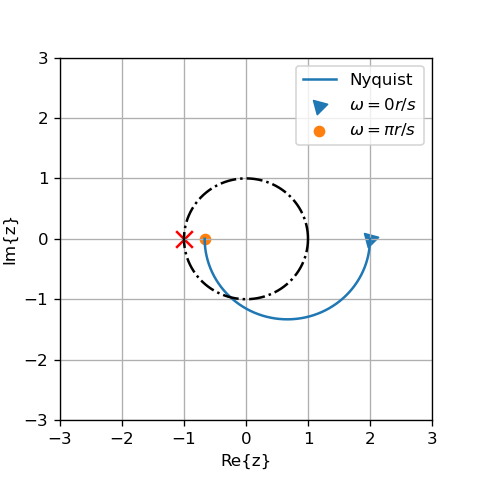
\includegraphics[width=.4\textwidth]{Img/7.png}
                \caption{Diagrama de Nyquist para la transferencia $H(z)$.}
                \label{}
            \end{figure}

            Como el sistema no encierra al punto $(-1;0)$ entonces $N=0$ y como $P=0$ ya que todos sus polos son estables el sistema permanecera. Si quisieramos controlar 
            el proceso con un proporcional las intersecciones con los ejes se darían en $2K$ y $-2K/3$, si tomamos $K>0$ podemos observar que el sistema sera 
            estable hasta que $N=1$ ya que la ni la planta ni el control poseen ceros por lo tanto $Z=0$ siempre. Luego como el sistema retroalimentado tiene 
            un unico polo para que el sistema sea estable tiene que suceder que $N=-P$ lo cual solo se da cuando $P=0$ por el sentido en la cual se recorre la curva.

            \begin{equation}
                -\frac{2K}{3} = -1 \Leftrightarrow K = \frac{3}{2}
            \end{equation}

            El diagrama de Nyquist para $K=3/2$ esta dado por:

            \begin{figure}[H]
                \centering
                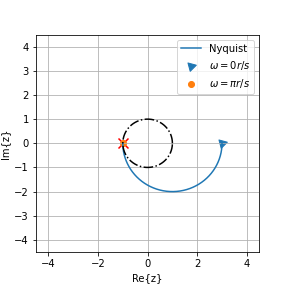
\includegraphics[width=.4\textwidth]{Img/7-1.png}
                \caption{Diagrama de Nyquist para $K=3/2$}
                \label{}
            \end{figure}

    \section{Ejercicio 8}
    
        \subsection{a)}

            En este caso la transferencia esta dada por 

            \begin{equation}
                H_1(z) = \frac{z-2}{z+2}
            \end{equation}

            Como primer paso analizaremos la ubicacion de los polos y ceros del sistema retroalimentado, es decir 

            \begin{equation}
                \label{eq:ej8-a}
                1 + KH_1(z) = 0 \Leftrightarrow z+2 + K(z-2) = 0 \Leftrightarrow z = 2 \frac{1 - K}{1 + K} 
            \end{equation}

            Podemos definir ciertos valores del criterio de establidad de Nyquist como que $P_0=1$, ya que el unico polo a lazo abiero se encuentra fuera del circulo unitario 
            y el controlador proporcional no agregar ninguno polo ni cero. 

            Primero calcularemos los valores de $K\in \mathcal{R}$ que hacen que el sistema sea inestable, por lo tanto:

            \begin{equation}
                |z| > 1 \Leftrightarrow
                2|1-K| > |1+K| 
            \end{equation}

            Si $K\leq-1$

            \begin{equation}
                2 - 2K > -1 - K \Leftrightarrow
                K < 3
            \end{equation}

            En este caso $Sol: K \in (-\infty;-1]$

            Para $-1<K<1$

            \begin{equation}
                2- 2K > 1+K  \Leftrightarrow
                1 > 3K \Leftrightarrow
                K < \frac{1}{3} 
            \end{equation}

            Para el segundo caso $Sol: K \in (-1; 1/3)$

            Por otro lado si $K\geq1$

            \begin{equation}
                -2 + 2K > 1 + K \Leftrightarrow
                K > 3
            \end{equation}

            Por ultimo $Sol: K \in ( 3; \infty )$

            La solución esta dada en la unión de los 3 intervalos luego el $P=1$ cuando $K \in (-\infty;1/3) \cup (3;\infty)$. Por lo tanto 
            el sistema sera estable cuando $K\in [ 1/3; 3 ]$.

            \begin{figure}[!htb]
                \centering
                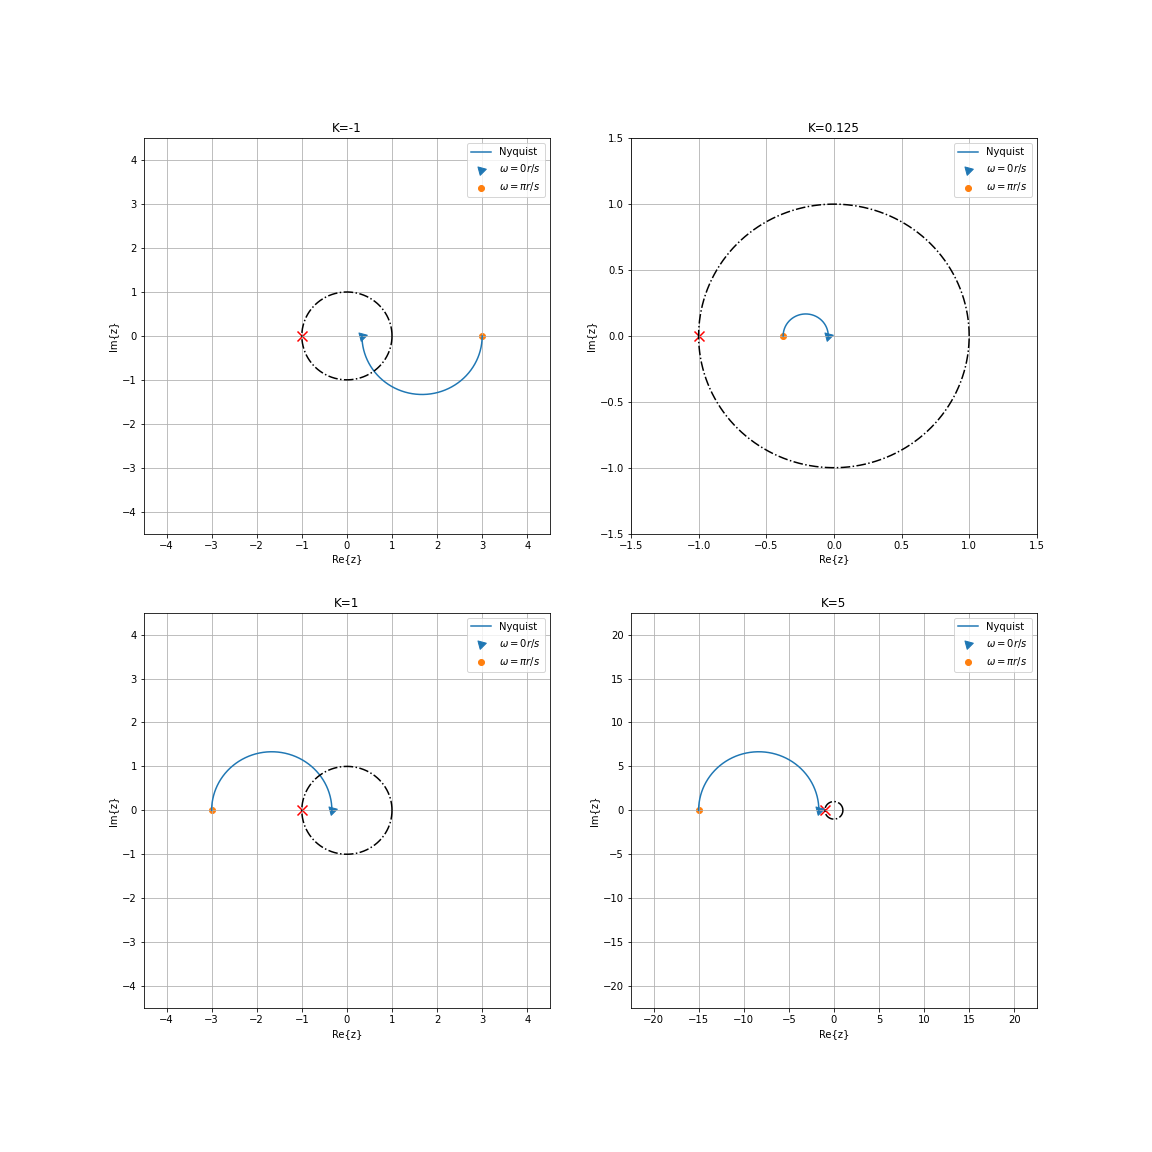
\includegraphics[width=\textwidth]{Img/8-a}
                \caption{Diagrama de Nyquist de $H_1(z)$ para distintos valores de $K$.}
                \label{fig:8-a}
            \end{figure}

            De los graficos presentados en la figura \ref{fig:8-a} es posible observar que cuando $K \notin [1/3;3]$ obtenemos que $N=0$ por lo 
            tanto $P_c=1$ y el sistema retroalimentado sera inestable. Por otro lado cuando $K \in [1/3 ;3]$ tenemos que el diagrama de Nyquist 
            rodea el punto $(-1;0)$ en sentido antihorario por lo cual $N=-1$ y el sistema retroalimentado es estable, ya que $P_c=0$.

        \subsection{b)}

            Para este ejercicio la transferencia esta dada por 

            \begin{equation}
                H_2(z) = \frac{1}{(z-2)(z+3)}
            \end{equation}
            
            Entonces si graficamos el lugar de las raices (figura \ref{fig:8-b-rlocus}) se obseva que el sistema retroalimentado sera estable mientras 
            se encuentre en un intervalo. 

            \begin{figure}[!htb]
                \centering
                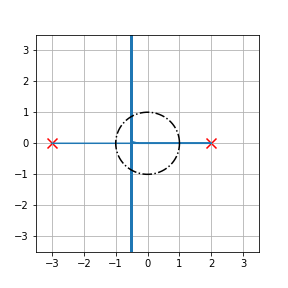
\includegraphics[width=.4\textwidth]{Img/8-b-rlocus.png}
                \caption{Lugar de las raices de $H_2(z)$.}
                \label{fig:8-b-rlocus}
            \end{figure}

            Para encontrar dichos limites utilizaremos el criterio de Jury. El polinomio caracterisco del sistema retroalimentado esta dado por 

            \begin{equation}
                P(z) = z^2 + z + ( K-6 )
            \end{equation}

            La tabla que se obtiene es 

            \begin{table}[H]
                \centering
                \begin{tabular}{|c|c|c|}
                    \hline $1$ & $1$ & $K-6$ \\
                    \hline $-K^2 +12K - 35$ & $7-K$ &  \\
                    \hline $\frac{-(K^2 - 12K -35)^2 + (K-7)^2}{K^2 - 12K -35}$ & & \\
                    \hline
                \end{tabular}
            \end{table}

            Ahora solo debemos calcular cuando 

            \begin{equation}
                1 > 0 \land - (K-7)(K-5) > 0 \land -\frac{(K-7)^2(K-6)(K-4)}{(K-7)(K-5)} > 0
            \end{equation}

            De las 2 primeras ecuaciones descriptas anteriormente se optiene que $K\in(6;7)$

            Si utlizamos el criterio de estabilidad de Nyquist debemos tenes en cuenta que como $P_0=2$ entonces $P_c=N + 2$, por lo tanto el 
            sistema sera estable cuando $N=-2$ ver figura \ref{fig:8-b-nyquist}

            \begin{figure}[!htb]
                \centering
                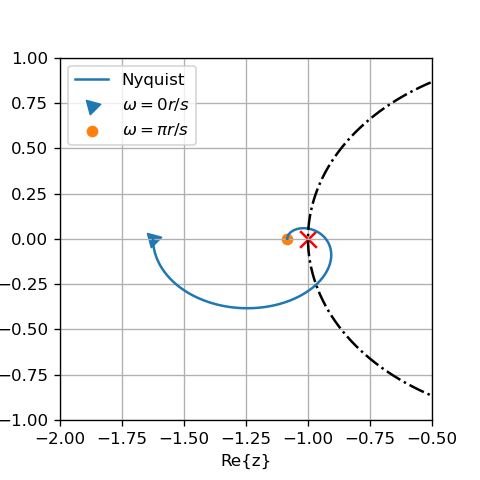
\includegraphics[width=.4\textwidth]{Img/8-b-nyquist}
                \caption{Diagrama de Nyquis para $K=6.5$ de $H_2(z)$.}
                \label{fig:8-b-nyquist}
            \end{figure}

        \subsection{c)}

        El proceso esta descripto por 

        \begin{equation}
            H_3(z) = \frac{4}{z^2 + 2z -1}
        \end{equation}

        Los polos del sistema a lazo abierto estan ubicados en $z \in \{ -1 \pm \sqrt{2}  \}$, luego $P_0=1$, por lo 
        tanto necesitaremos que $N=-1$. De la figura \ref{fig:8-c-nyquist} podemos observar que $N=1$ por lo tanto si 
        cerramos el lazo con $K=1$ el sistema tendra 2 polos fuera del circulo unitario. Tambien es posible determinar 
        que $H(1) = 2K$ y $H(-1)=-2K$, por lo tanto siempre encerraremos al valor $(-1;0)$ si $|K|>1/2$ con el mismo sentido 
        por lo tanto el sistema no es estable para ningun $K \notin (-1/2 ; 1/2)$. Ahora solo nos falta analizar que 
        pasa cuando $|K|<1/2$, debido a que la curva se contrae las intersecciones quedan dentro del circulo unitario 
        y por lo tanto no es posible encerrar al $(-1;0)$. Como conclución podemos decir que no es posible controlar 
        este proceso con un control proporcional.

        \begin{figure}[!htb]
            \centering
            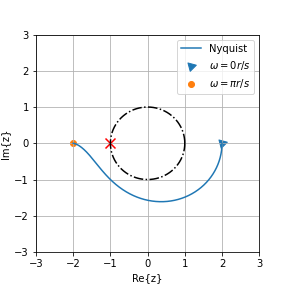
\includegraphics[width=.4\textwidth]{Img/8-c-nyquist}
            \caption{Diagrama de Nyquist de $H_3(z)$ para $K=1$.}
            \label{fig:8-c-nyquist}
        \end{figure}

        El grafico del lugar de las raices, es bastante sencillo y se puede observar que nunca se encuentran ambos polos dentro del circulo 
        unitario, lo cual es razonable segun el analisis hecho anteriormente.

    \section{Ejercicio 9}

        La transferencia del proceso esta dada por 

        \begin{equation}
            H(z) = \frac{1}{z(z - 1/2)}
        \end{equation}

        \subsection{a)}

        Al utilizar un controlador proporcional sabemos que el numero de polos y ceros del sistema no varia por lo tanto 
        como ambos polos tienen polos menores a $1$ entonces $P_c=0$ por lo tanto no debemos encerrar al punto $(-1;0)$ con el diagrama de Nyquist para que el sistema 
        sea estable. En la figura \ref{fig:9-a-nyquist} se puede observar que las intersecciones con el eje real quedan determinas por $-K$ y $2K$, 
        podemos plantear que el diagrama de Nyquist nunca encerrara al $(-1;0)$ cuando este no este contenido en el intervalo $(-K;2K)$, el caso limite se 
        da cuando 

        \begin{equation}
            -K=-1 \lor 2K=-1
        \end{equation}

        Ya que en dichos casos los bordes de la curva de Nyquist caen en $-1$, por lo tanto $K \in (-1/2;1)$ como $K>0$ entonces $K \in (0;1)$.

        \begin{figure}[!htb]
            \centering
            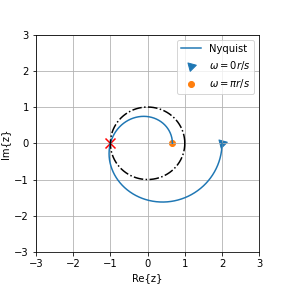
\includegraphics[width=.5\textwidth]{Img/9-a.png}
            \caption{Diagrama de Nyquist de $H(z)$ con un control proporcional para $K=1$.}
            \label{fig:9-a-nyquist}
        \end{figure}

        Llegariamos al mismo resultado si planteamos el criterio de estabilidad de Jury, solo que el procedimiento es un poco mas engorroso.

        Luego el error en estado estacionario esta dado por 

        \begin{equation}
            \lim_{ k \to \infty } e[k] = \lim_{z \to 1} (1 - z^{-1}) \frac{z^2 - z/2}{z^2 - z/2 + K} \frac{1}{1 - z^{-1}} = \frac{3}{1 + 2K}
        \end{equation}

        \subsection{b)}

        Si controlamos la planta con un integral tenemos que la transferencia $H_1(z)$ en lazo abierto esta descripta por 

        \begin{equation}
            H_1(z) = \frac{K}{(z-1)(z-1/2)}
        \end{equation}

        Al igual que el caso anterior ambos polos se encuentran dentro o en el borde de la region de estabilidad, por lo tanto $P_c=0$. Luego 
        el requisito para que a lazo cerrado el sistema sea estable es que $N=0$. En la figura \ref{fig:9-b-nyquist} podemos observar 
        el diagrama de Nyquist para $K=1$ y obtenemos que las intersecciones con el eje real se dan en $-2K$ y en $K/3$. Al 
        igual que el inciso anterior el caso limite se da cuando una de las intersecciones cae sobre el $-1$ con 
        lo que obtenemos que $K=1/2$ y $K=-3$, sabiendo que $K>0$ y que no el desplazamiento logrado para $K>1/2$ haría que 
        la interseccion sea hacia la izquierda del $-1$, lo cual indicaría el sistema es inestable ya que $N=1$.

        \begin{figure}[!htb]
            \centering
            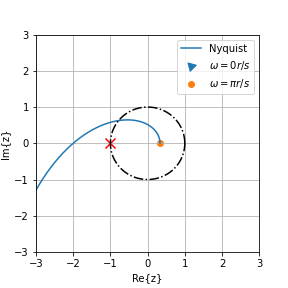
\includegraphics[width=.5\textwidth]{Img/9-b-nyquist.png}
            \caption{Diagrama de Nyquist para $K=1$ de $H_1(z)$.}
            \label{fig:9-b-nyquist}
        \end{figure}

        Realizando el mismo planteo que el inciso anterior 

        \begin{equation}
            \lim_{k \to \infty} e[k] = 
            \lim_{z \to 1} (1 - z^{-1}) \frac{z^2 - 3z/2 + 1/2}{z^2 - 3z/2 + 1/2 + K} \frac{1}{1-z^{-1}} = 0
        \end{equation}

    \section{Ejercicio 10}

        \subsection{a)}

            Para el control proporcional tenemos que $K \in (0;1)$, el error para una rampa esta dado por 

            \begin{equation}
                \lim_{k \to \infty} e[k] = \lim_{z \to 1} (1 - z^{-1}) \frac{z^2 - z/2}{z^2 - z/2 + K} \frac{z^{-1}}{(1-z^{-1})^2}
                = \lim_{z \to 1} \frac{(z-1/2)}{(z^2 - z/2 + K)(1-z^{-1})} \to \infty
            \end{equation}
    
            Debido a que la entrada no es acodata y en este caso la salida tambien diverge no es posible determinar el error en 
            estado estacionario de una rampa.

        \subsection{b)}

            En el caso del control integral obtenemos que el error para una rampa esta dado por 

            \begin{equation}
                \lim_{k \to \infty} e[k] = \lim_{z \to 1} (1 - z^{-1}) \frac{z^2 - 3z/2 + 1/2}{z^2 - 3z/2 + 1/2 + K} \frac{z^{-1}}{(1-z^{-1})^2}
                = \lim_{z \to 1} \frac{z-1/2}{z^2 -3z/2 + 1/2 + K} = \frac{1}{2K} 
            \end{equation}

            El error minimo se obtiene para el maximo valor de $K$, en el ejercicio anterior se determino que el maximo valor de $K$ posible es $1/2$. 
            En ese caso el error obtenido es $1$.

    \section{Ejercicio 11}

        En este caso la transferencia del proceso esta descripta por 
        
        \begin{equation}
            H(z) = \frac{5}{z( 5z + 2 )}
        \end{equation}

        \subsection{a)}

            Si controlamos con un proporcional la transferencia a lazo abierto que se obtiene es 

            \begin{equation}
                H_1(z) = \frac{5K}{z(5z+2)}
            \end{equation}

            Como ambos polos se encuentran dentro del circulo unitario entonces $P_0=0$, por lo tanto necesitaremos que $N=0$ para 
            que el sistema a lazo cerrado sea estable. Calcularemos las intersecciones de $H_1(z)$ con el eje real. 

            \begin{equation}
                \arg \{ H_1(e^{j\omega}) \} = k\pi, k \in \mathbb{R^+}
            \end{equation}

            Por lo tanto 

            \begin{equation}
                \arg \{ 5 \} + \arg\{K \}  - \arg\{ 5e^{2j\omega} + 2e^{j\omega} \} = k\pi
            \end{equation}

            En el caso de que $K>0$ entonces 

            \begin{equation}
                - \arg\{ 5\sin{2\omega} + 2\sin{\omega}+ 5\cos{2\omega} + 2\cos{\omega} \} = k\pi
            \end{equation}

            De la ecuación podemos determiar que las intercciones se daran cuando $5\sin{2\omega} + 2\sin{\omega}= 0$. 

            \begin{equation}
                5\sin{ 2\omega } + 2\sin{ \omega } = 0
            \end{equation}

            Existen soluciones triviales a esta ecuaciones y son cuando $\omega$ es un multiplo de $\pi$, como la el intervalo de interes esta 
            dado entre $[0;\pi]$ nos quedaremos con 2 soluciones triviales $\omega \in \{ 0, \pi \}$. Por ultimo nos queda determinar la existencia de 
            otras soluciones 
            
            \begin{equation}
                \sin\{ \omega \}( 10\cos{ \omega } + 2 ) = 0 \Leftrightarrow
                10\cos{ \omega } = -2 \Leftrightarrow
                \cos{ \omega } = -\frac{1}{5} \Leftrightarrow
                \omega \approx 1.77 rad
            \end{equation}

            Si aluamos $H_1(z)$ obtendremos los valores de las intercciones, las cuales se dan en 


            \begin{table}[H]
                \centering 
                \begin{tabular}{|c|c|c|c|}
                    \hline $\omega$ & $0$ & $\pi$ & $\arccos{-\frac{1}{5}}$ \\ 
                    \hline $H(e^{j\omega})$ & $\frac{5K}{7}$ & $\frac{5K}{3}$ & $-K$ \\
                    \hline
                \end{tabular}
            \end{table}

            En la figura \ref{fig:11-nyquist} se observa la curva de Nyquist para $K=1$ y se observan las 3 intersecciones calculadas anteriormente.
            Luego para que $N=0$ el punto $(-1;0)$ no debe estar contenido en el interior de la curva por lo tanto podemos plantear que 

            \begin{equation}
                \frac{5K}{7} = -1 \land \frac{5K}{3} = -1 \land -K = -1 \Leftrightarrow
                K = -\frac{7}{5} \land K = -\frac{3}{5} \land K = 1
            \end{equation}

            Luego estos son los valores donde cada una de las intersecciones cae sobre el $-1$, por lo tanto para que nunca se encierre dicho 
            valor debemos excluir los intervalor que hagan que la interseccion quede a la izquierda del $-1$, en los 2 primeros casos se da cuando 
            $K$ es menor al valor limite, mientras que en el ultimo caso se da cuando $K$ es mayor al valor limite, por lo que obtenemos que $K \in (-3/5;1)$.
            En caso de utilizar $K>0$ tendremos que $K \in (0;1)$.

            \begin{figure}[!htb]
               \centering
               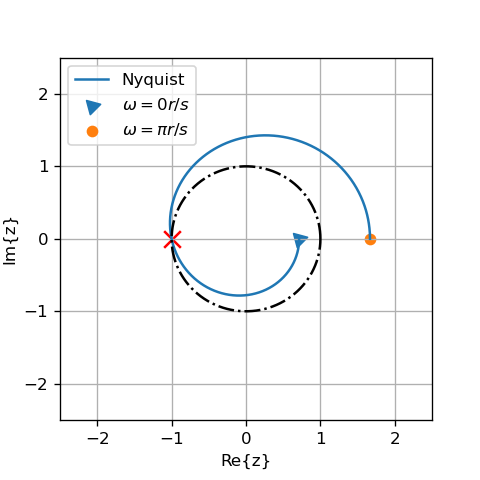
\includegraphics[width=.5\textwidth]{Img/11-nyquist.png}
               \caption{Diagrama de Nyquist de $H_1(z)$ para $K=1$.}
               \label{fig:11-nyquist}
            \end{figure}

        \subsection{b)}

            Como para $K=0.5$ el sistema es estable podemos calcular el error en estado estacionario. El cual se puede determinar utilizando la transformada $Z$.

            \begin{equation}
                \lim_{k \to \infty} e[k] = \lim_{z \to 1} (1-z^{-1}) \frac{1}{1 + \frac{5K}{z(5z + 2)}} \frac{1}{z^{-1}} \Leftrightarrow
                \lim_{k \to \infty} e[k] = \lim_{z \to 1} \frac{z(5z+2)}{5z^2 + 2z + 5K} \Leftrightarrow
                \lim_{k \to \infty} e[k] = \frac{14}{19}
            \end{equation}

    \section{Ejercicio 12}
    
        La planta a lazo abieto puede ser expresada como 
        
        \begin{equation}
            H_p(z) = \frac{4(z+2)}{10z^2 - 12z + 5}
        \end{equation}

        Si controlamos con un controlado $H_c(z)$ descripto por 
        
        \begin{equation}
            H_c(z) = -K
        \end{equation}

        Suponiendo que retroalimentamos positivamente, lo cual es equivalente a retroalimentar de forma negativa utilizando el controlador 
        
        \begin{equation}
            H_c(z) = K
        \end{equation}

        Tenemos que la planta mas el controlador queda expresado como 

        \begin{equation}
            H(z) = \frac{4K(z+2)}{10z^2 - 12z +5}
        \end{equation}

        El diagrama de Nyquist puede verse en la figura \ref{fig:12-nyquist}, en la cual se observan 3 intersecciones con el eje real. 
        Para obtener dichas intersecciones veremos cuando $\arg\{H(z)\} = k\pi, k \in \mathbb{R}$. Pero antes notemos que si mutiplico y
        divido $H(z)$ por $\bar{(z+2)}$ obtenemos 

        \begin{equation}
            H(z) = \frac{4K|z+2|^2}{(10z^2 - 12z +5)(\bar{z} + 2)}
        \end{equation}

        Este planteo nos simplificara las cuentas mas adelante, ya que para realizar el diagrama de Nyquist debemos tomar $z=e^{j\omega}$, por lo tanto 
        $z\bar{z}=1$. Finalmente 


        \begin{equation}
            \arg\{ 4K \} + \arg \{ |z+2|^2\} - \arg \{ (10z^2 - 12z +5)(\bar{z} + 2) \}= k\pi
        \end{equation}

        Sabemos que el argumento de un numero positivo es nulo y el argumento de $K$ es $\pi$ cuando $K<0$ o $0$ si $K\geq0$ por lo tanto obtenemos que 


        \begin{equation}
            - \arg \{ (10z^2 - 12z +5)(\bar{z} + 2) \} = ( k - \mu(-K) ) \pi
        \end{equation}

        Desarrollando la expresión $(10z^2 - 12z +5)(\bar{z} + 2)$ obtenemos que 

        \begin{equation}
            (10z^2 - 12z +5)(\bar{z} + 2) = 10z^2\bar{z} + 20z^2 -12z\bar{z} - 24z + 5\bar{z} + 10 \Leftrightarrow
            (10z^2 - 12z +5)(\bar{z} + 2) = 20z^2 - 14z + 5\bar{z} - 2
        \end{equation}

        Por lo tanto si tomamos $z=e^{j\omega}$ e igulamos la parte imaginaria a $0$, que es lo que determina cuando $\arg\{ H(z) \}$ es un 
        multiplo de $\pi$. 

        \begin{equation}
            20\sin{ 2\omega } - 14\sin{ \omega } - 5\sin{ \omega } = 0 \Leftrightarrow
            \sin{ \omega }( 40\cos{ \omega } - 19 ) = 0 \Leftrightarrow
            \omega = 0 \lor \omega = \pi \lor \omega = \arccos\left( \frac{19}{40} \right)
        \end{equation}

        \begin{figure}
            \centering
            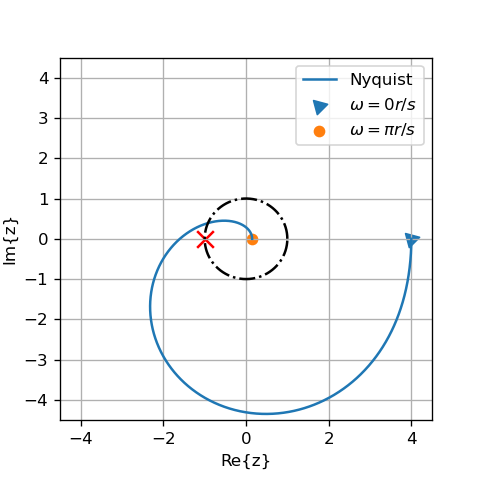
\includegraphics[width=.5\textwidth]{Img/12-nyquist.png}
            \caption{Diagrama de Nyquiste de $H(z)$ para $K=1$.}
            \label{fig:12-nyquist}
        \end{figure}

        Ahora debemos terminar el valor de $H(z)$ para los puntos determinados, lo cual es simplemente remplazar $z=e^{j\omega}$.

        \begin{table}[H]
            \centering
            \begin{tabular}{|c|c|c|}
                \hline $0$ & $\pi$ & $\arccos{19/40}$ \\ 
                \hline $8K/5$ & $4K/27$ & $-8K/5$ \\
                \hline
            \end{tabular}
        \end{table}

        Luego como $N=0$ para que el sistema a lazo cerrado sea estable las todas las intersecciones deben estar en la región 
        derecha o izquierda del $-1$. Lo cual sucedera cuando 

        \begin{equation}
            \frac{8}{5}K > -1 \land \frac{4}{27}K > -1 \land -\frac{8}{5}K > -1 \Leftrightarrow
            K > -\frac{5}{8} \land K > -\frac{4}{27} \land K < \frac{5}{8}
        \end{equation}
        
        Como en este caso si plantemos $<$ en vez de $>$ la solución es vacío solo se desarrollo en el caso de interes. 
        Por lo tanto el sistema resulta estable cuando $K \in (-4/27;5/8)$, si tomamos $K>0$ entonces $K \in( 0 ; 5/8 )$.
        Con la finalidad de comprobar el planteo se muestra en la figura \ref{fig:12-rlocus} el lugar de las raíces.

        \begin{figure}
            \centering
            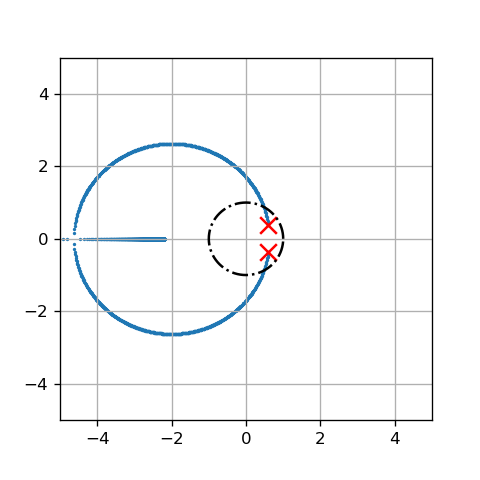
\includegraphics[width=.5\textwidth]{Img/12-rlocus.png}
            \caption{Lugar de las raíces de $H(z)$}
            \label{fig:12-rlocus}
        \end{figure}

\end{document} 
